Cette Section a pour but d'utiliser au mieux l'outil de MCRT. La première sous partie valide la stratégie de vectorisation utilisée dans \ttt{EMBREE} qui permet de d'accélérer les calculs d'un facteur 10 sur certaines machines. La seconde sous partie traite de la parralélisation du code grâce à la libraire \ttt{TBB} qui permet d'utiliser au mieux les différents procésseurs de la machine utiliser avec un taux d'accélération \red{insert value}.
\subsection{Amélioration des performances du code}
\subsubsection{Vectorisation des rayons grâce à \texttt{EMBREE}}
Afin d'évaluer l'intérêt du traitement des rayons par paquets, une étude de performances a été menée en faisant varier la taille des paquets de 1 à 16 rayons. Les temps d'exécution obtenus pour différents nombres de rayons sont présentés à la Figure~\ref{fig:packet_time}, tandis que le Tableau~\ref{tab:packet_perf} récapitule les performances mesurées. Quelle que soit la taille des paquets, les temps de calcul évoluent linéairement avec le nombre de rayons, comme l'illustre la droite de référence de pente un. Ce résultat confirme que le coût de l'algorithme est essentiellement proportionnel au nombre de rayons simulés.

L'amélioration des performances observée lorsque la taille des paquets augmente provient de la stratégie de vectorisation employée par la bibliothèque \texttt{Embree}. Plutôt que de traiter chaque rayon indépendamment, plusieurs rayons sont regroupés afin d'exploiter les unités de calcul vectoriel (SIMD, \textit{Single Instruction Multiple Data}) des processeurs modernes. Cette approche permet d'appliquer simultanément les opérations de traversée de la hiérarchie BVH et les tests d'intersection à plusieurs rayons, réduisant ainsi le coût moyen de traitement par rayon. La bibliothèque sélectionne automatiquement les noyaux de calcul les mieux adaptés aux capacités vectorielles du processeur (SSE, AVX ou AVX2 dans notre cas), tout en conservant une interface de programmation indépendante de l'architecture matérielle. Les gains observés ne résultent donc pas uniquement de l'exécution simultanée de plusieurs opérations, mais également d'une meilleure utilisation de la hiérarchie mémoire et d'un amortissement du coût de traversée des structures d'accélération. 

Les simulations ont été réalisées sur une station de calcul équipée de deux processeurs Intel Xeon E5-2630~v4 (20 cœurs physiques, 40 fils d'exécution) supportant les instructions AVX2. Sur cette architecture, une taille de paquet de 16 rayons offre les meilleures performances. Pour un million de rayons, le temps d'exécution est réduit d'un facteur supérieur à 10 par rapport au traitement rayon par rayon, ce qui met en évidence l'intérêt de cette stratégie de vectorisation pour les simulations Monte Carlo de transfert radiatif.

\begin{table}[ht]
\centering


\begin{tabular}{ccc}
\toprule
Taille du paquet & Temps (ms) pour $10^6$ rayons & Speedup \\
\midrule
1  & 439\,561 & 1.00 \\
2  & 229\,972 & 1.91 \\
4  & 125\,643 & 3.50 \\
8  &  71\,149 & 6.18 \\
16 &  43\,593 & 10.08 \\
\bottomrule
\end{tabular}
\caption{Temps d'exécution (ms) en fonction de la taille des paquets de rayons. Le facteur d'accélération est calculé par rapport au traitement rayon par rayon ($N_p=1$).}
\label{tab:packet_perf}
\end{table}


\subsubsection{Accéleration du lancer de rayons en utilisant la Bounding Volume Hierarchy}

Dans une simulation de lancer de rayons, la majeure partie du temps de calcul est consacrée à la recherche des intersections entre les rayons et la géométrie. Une approche naïve consisterait à tester chaque rayon contre l'ensemble des triangles du maillage. Pour une scène composée de $N$ triangles, cette méthode nécessite jusqu'à $N$ tests d'intersection par rayon, ce qui devient rapidement prohibitif pour les géométries industrielles.

Afin de réduire ce coût, la bibliothèque \textsc{Embree} construit automatiquement une \emph{Bounding Volume Hierarchy} (BVH), c'est-à-dire une hiérarchie de volumes englobants contenant les éléments du maillage. Chaque nœud de cette hiérarchie est associé à une boîte englobante (\emph{Axis-Aligned Bounding Box}, AABB) qui renferme un sous-ensemble des triangles de la scène. Les feuilles de l'arbre contiennent finalement les triangles sur lesquels sont réalisés les tests d'intersection précis.

Lors du lancer d'un rayon, l'intersection est d'abord évaluée avec la boîte englobante de la racine. Si le rayon ne traverse pas une boîte fille, l'ensemble des triangles qu'elle contient est immédiatement écarté, sans qu'aucun test supplémentaire ne soit effectué. À l'inverse, seules les branches effectivement traversées par le rayon sont explorées récursivement jusqu'aux feuilles de l'arbre. Cette stratégie permet d'éliminer très rapidement de grandes portions de la géométrie et de limiter les calculs aux seuls triangles susceptibles d'être rencontrés.

L'utilisation d'une BVH réduit ainsi considérablement le nombre de tests d'intersection nécessaires. En pratique, le coût moyen de recherche d'une intersection devient proche d'une croissance logarithmique avec le nombre de triangles, contre une croissance linéaire pour une recherche exhaustive. Cette amélioration constitue l'une des principales raisons des excellentes performances de la bibliothèque \textsc{Embree} pour le lancer de rayons.

\begin{figure}[H]
    \centering
    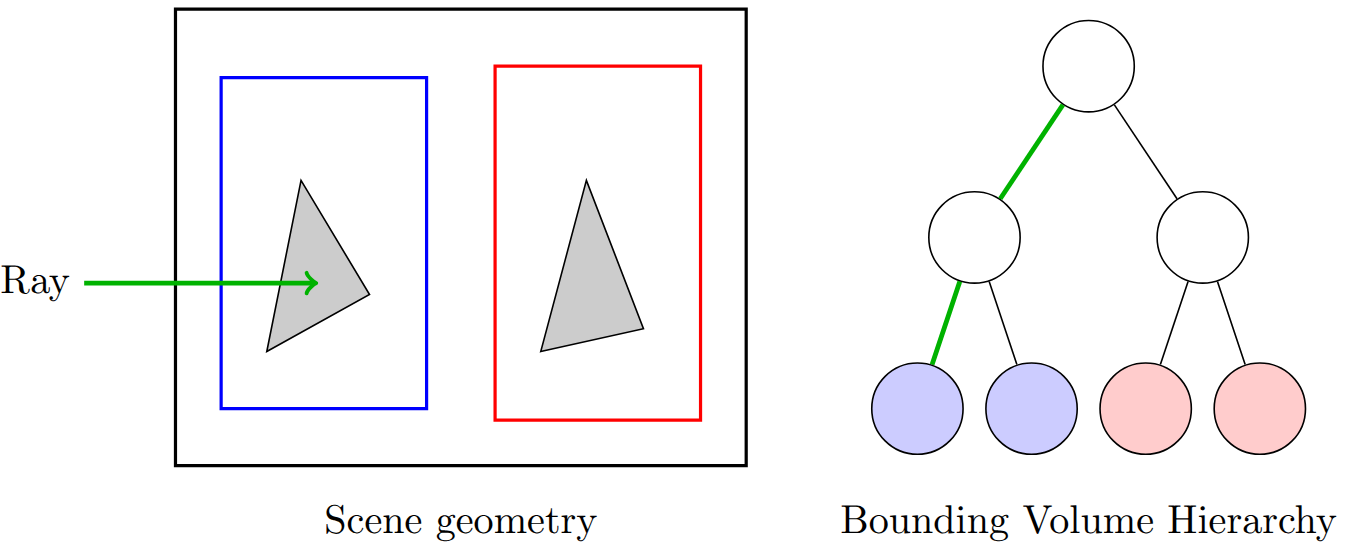
\includegraphics[width = \linewidth]{PICTURES/c2/bvh.png}
    \caption{Illustration du BVH}
    \label{fig:bvh}
\end{figure}

\subsubsection{Parallélisation du code avec la librairie \ttt{TBB}}



\subsection{Optimisation de la variance liée à la répétition des simulations}


\subsection{Stratégie à suivre pour des géométries 2D}
comparaison 2D et 3D infini

